% !TEX root = main.tex
% === ハードウェア ==========================================================

\subsection{ハードウェア構成}
本システムのハードウェア構成について,以下に各要素を説明する.

\subsubsection{マイコン(STM32 Nucleo Board STM32F446RE)}
本システムでは,STM32 Nucleo Board STM32F446REマイコンボードを使用している.
STM32 F446REは高性能なARM Cortex-M4プロセッサを搭載しており,以下の特徴を持つ.
\begin{itemize}
    \item 最大180 MHzのクロック速度
    \item タイマーをエンコーダモードに設定可能
    \item 開発/評価ボードであり入手性が高い
\end{itemize}
本マイコンは,モーター駆動,エンコーダーのデータ取得を担当しており,
ロボットの下位制御レイヤーを実現している.


\subsubsection{エンコーダー(AMT102-V)}
AMT102-Vエンコーダーを採用し,モーターの回転角速度および回転位置を計測している.
図\ref{fig:AMT102}に使用するエンコーダーを示す.
このエンコーダーは最大分解能は2048 PPR(Pulse Per Revolution)であり,
非接触方式である.
エンコーダーからの信号はマイコンで処理され,
車輪の速度制御や自己位置推定に使用する.

\begin{figure}[H]
    \centering
    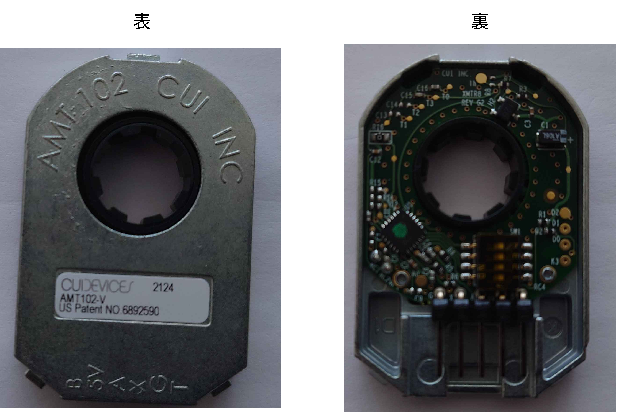
\includegraphics[width=0.5\textwidth]{figure/AMT102.pdf}
    \caption{AMT102-V}
    \label{fig:AMT102}
\end{figure}

\subsubsection{深度カメラ(Intel RealSense D435i)}
深度カメラとしてIntel RealSense D435iを採用している.D435iは,ステレオカメラ方式に基づく高精度な距離計測を特徴とし,以下のような仕様を持つ.
\begin{itemize}
    \item 最大測定距離:0.1~10メートル
    \item フレームレート:最大90 FPS
    \item 視野角:水平87°,垂直58°
    \item IMU(慣性計測ユニット)搭載
\end{itemize}
本システムでは,D435iから取得した深度データを用いて目標(人)の位置を検出し,
追従アルゴリズムに利用している.

\begin{figure}[H]
    \centering
    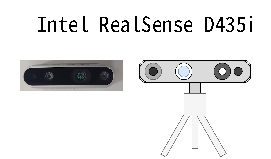
\includegraphics[width=0.5\textwidth]{figure/RealSense.pdf}
    \caption{RealSense}
    \label{fig:RealSense}
\end{figure}

D435iの内部パラメータ(焦点距離と光学中心)は,以下のPythonコードを使用して計測した.

\begin{lstlisting}[language=Python, caption=RealSense内部パラメータの取得]
import pyrealsense2 as rs

# RealSenseパイプラインのセットアップ
pipeline = rs.pipeline()
config = rs.config()
config.enable_stream(rs.stream.depth, 640, 480, rs.format.z16, 30)
pipeline.start(config)

# 深度ストリームのプロファイルからカメラパラメータを取得
profile = pipeline.get_active_profile()
depth_stream = profile.get_stream(rs.stream.depth)  # 深度ストリーム
intrinsics = depth_stream.as_video_stream_profile().get_intrinsics()

# 内部パラメータを取得
fx = intrinsics.fx  # 焦点距離 (f_x)
fy = intrinsics.fy  # 焦点距離 (f_y)
cx = intrinsics.ppx  # 光学中心 x座標 (c_x)
cy = intrinsics.ppy  # 光学中心 y座標 (c_y)

print(f"焦点距離: fx={fx}, fy={fy}")
print(f"光学中心: cx={cx}, cy={cy}")

# 使用後はパイプラインを停止
pipeline.stop()
\end{lstlisting}

このコードを実行した結果,D435iの焦点距離と光学中心が以下の通り得られた.

\begin{itemize}
    \item 焦点距離:$f_x = 378.09$ [pixel],$f_y = 378.09$ [pixel]
    \item 光学中心:$c_x = 319.39$ [pixel],$c_y = 237.10$ [pixel]
\end{itemize}

これらの内部パラメータは,ピクセル座標系からカメラ座標系への変換(式\eqref{eq:xc},\eqref{eq:yc})で使用される.